

After discretising the domain in {\python nel} elements, and having decided the FE
pair we want to use to solve the Stokes equations (in this case \QtwoQone), we end up 
having to compute elemental integrals such as 
\[
\K_e = \int_{\Omega_e} {\bm B}^T\cdot {\bm C}_\eta \cdot {\bm B} \; d\Omega
\]
where $\Omega_e$ denotes an element.
The way we carry out this integration is by means of the Gauss-Legendre quadrature, which 
forces us to carry out a change of variables from the original element $\Omega_e$ 
to the reference element $(r,s) \in [-1,1]\times [-1,1]$. For this we establish a mapping between both 
as explained in Section 7.13 of fieldstone.
Basis functions $Q_{1,2,3,4}$ are defined in Section 3.4.

\begin{center}
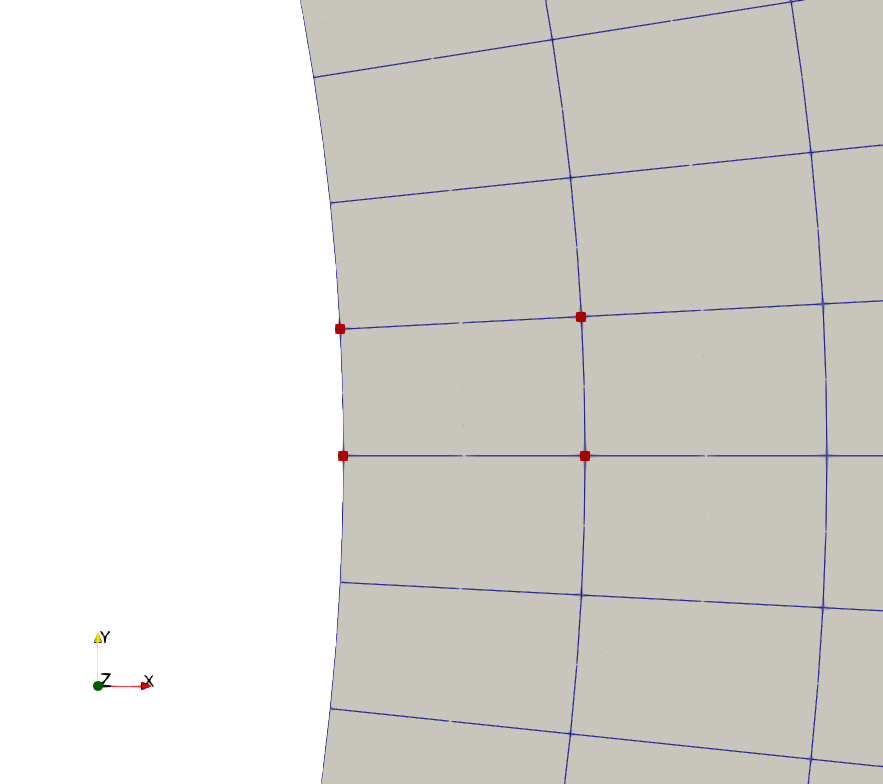
\includegraphics[width=4.2cm]{images/mappingQ1}
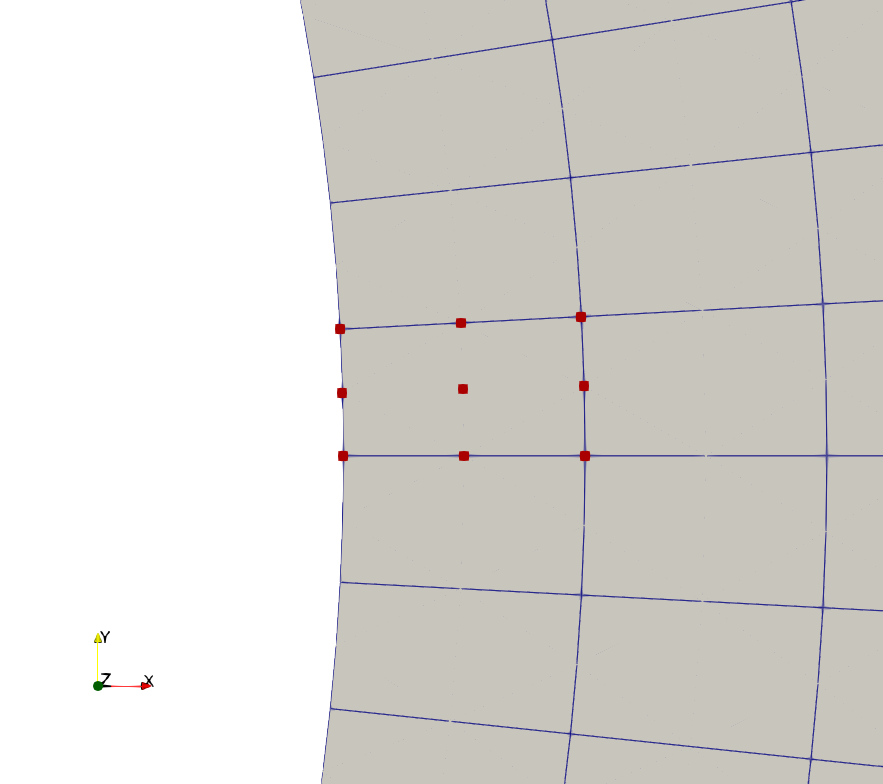
\includegraphics[width=4.2cm]{images/mappingQ2}
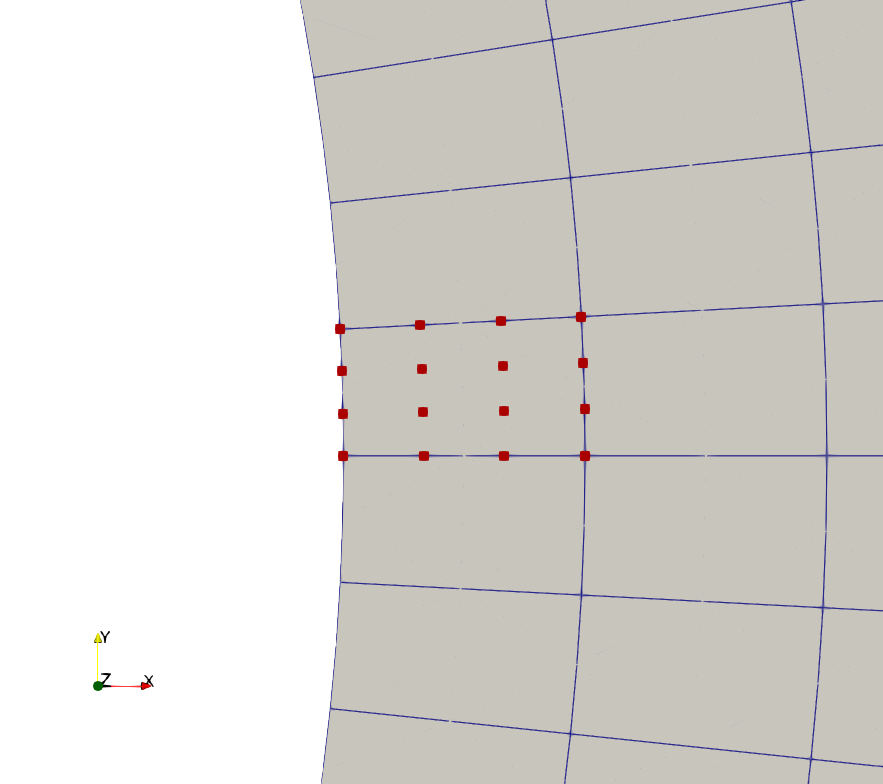
\includegraphics[width=4.2cm]{images/mappingQ3}
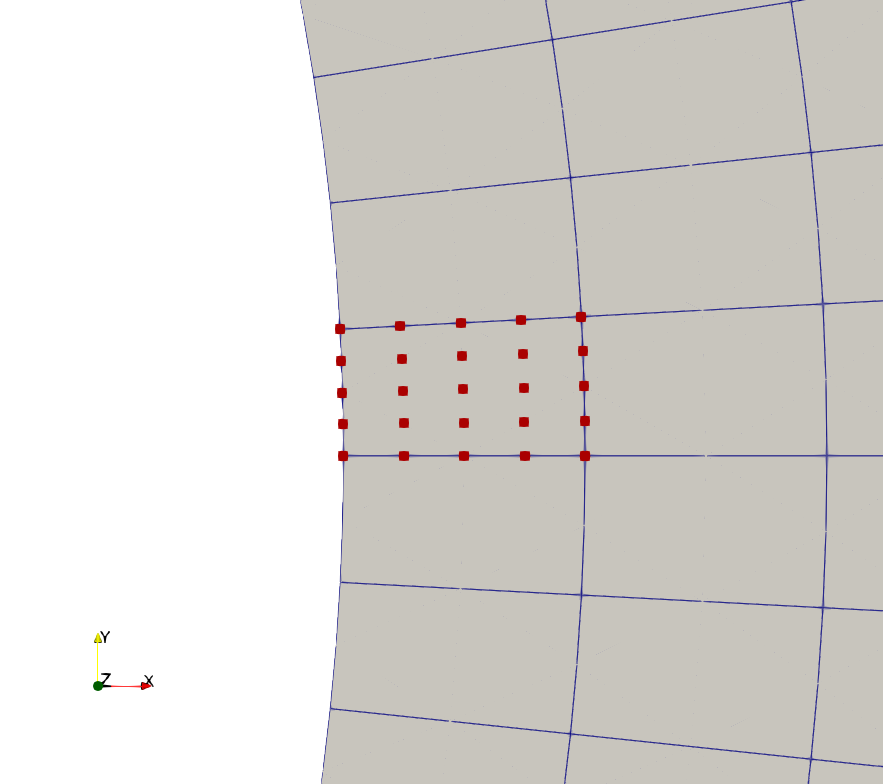
\includegraphics[width=4.2cm]{images/mappingQ4}\\
{\captionfont Layout of the mapping nodes in element \#0 of the mesh. 
From left to right: $Q_1$, $Q_2$, $Q_3$ and $Q_4$. Rows of nodes are placed 
on concentric circles and columns of nodes are equidistant in $\theta$ space.} 
\end{center}

For each element we store the coordinates of these mapping points into two 
arrays:
\begin{lstlisting}
xmapping=np.zeros((X,nel),dtype=np.float64)
ymapping=np.zeros((X,nel),dtype=np.float64)
\end{lstlisting}
where {\python X} stands for the number of nodes for each mapping.

The reduced coordinates for the quadrature points are given by 
the Gauss-Legendre quadrature approach. The real coordinates of these points
is a function of the mapping used so that 
\begin{lstlisting}
for iel in range(0,nel):
    for kq in range(0,nqel):
        rq=qcoords_r[kq]
        sq=qcoords_s[kq]
        NNNV=NNN(rq,sq,mapping)
        xq=np.dot(NNNV[:],xmapping[:,iel])
        yq=np.dot(NNNV[:],ymapping[:,iel])
\end{lstlisting}
Likewise the Jacobian matrix is by definition a function of the chosen mapping 
so that 
\begin{lstlisting}
for iel in range(0,nel):
    for kq in range(0,nqel):
        rq=qcoords_r[kq]
        sq=qcoords_s[kq]
        dNNNVdr=dNNNdr(rq,sq,mapping)
        dNNNVds=dNNNds(rq,sq,mapping)
        jcb[0,0]=np.dot(dNNNVdr[:],xmapping[:,iel])
        jcb[0,1]=np.dot(dNNNVdr[:],ymapping[:,iel])
        jcb[1,0]=np.dot(dNNNVds[:],xmapping[:,iel])
        jcb[1,1]=np.dot(dNNNVds[:],ymapping[:,iel])
        jcob=np.linalg.det(jcb)
        jcbi=np.linalg.inv(jcb)
\end{lstlisting}


\begin{center}
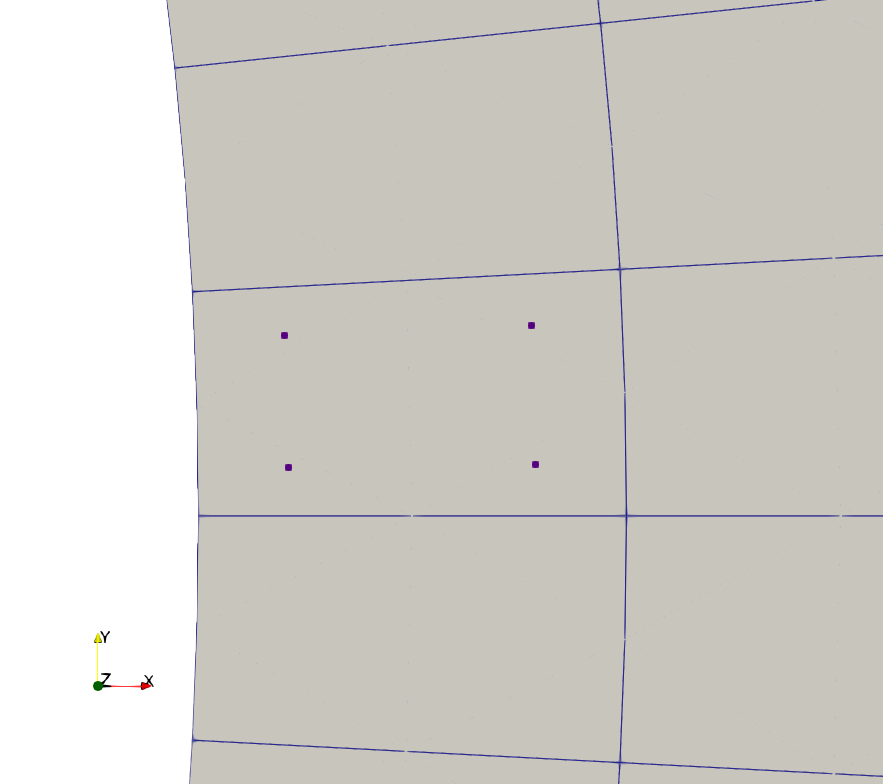
\includegraphics[width=4.2cm]{images/nq4}
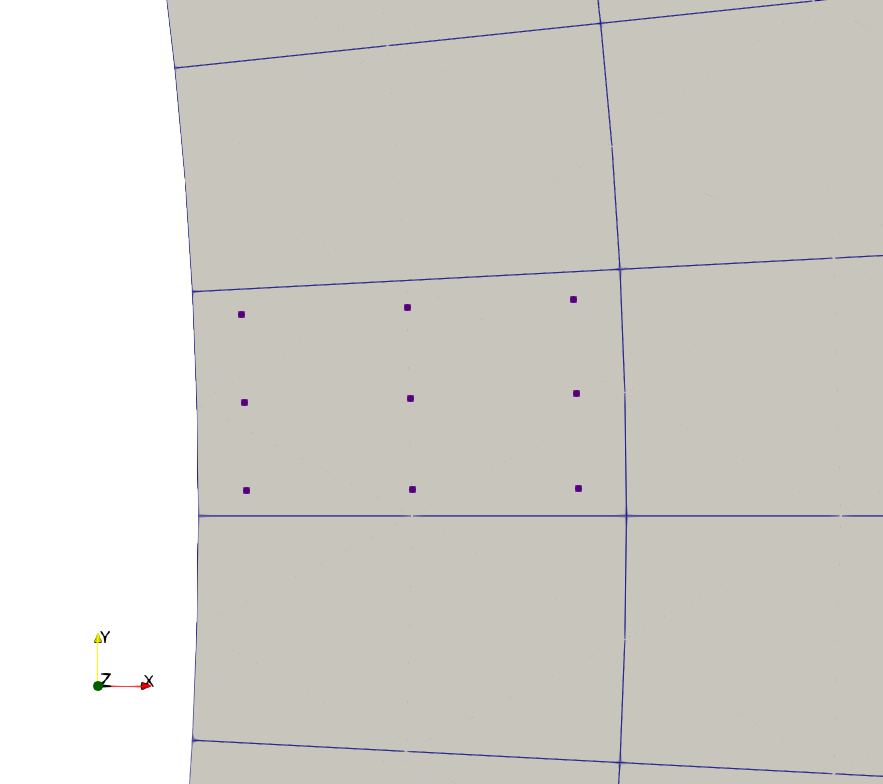
\includegraphics[width=4.2cm]{images/nq9}
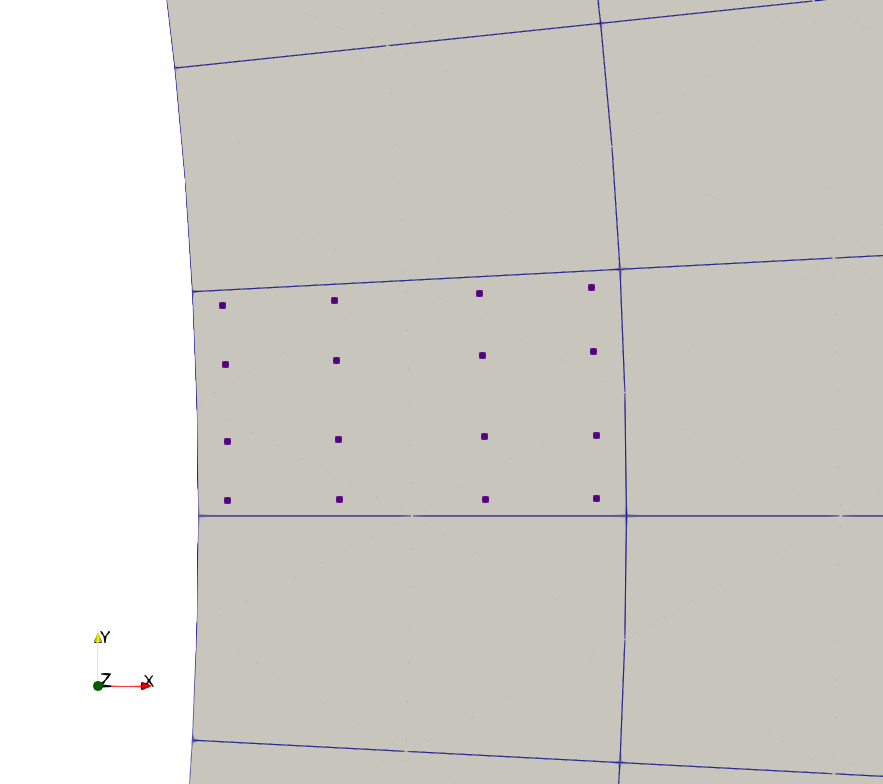
\includegraphics[width=4.2cm]{images/nq16}
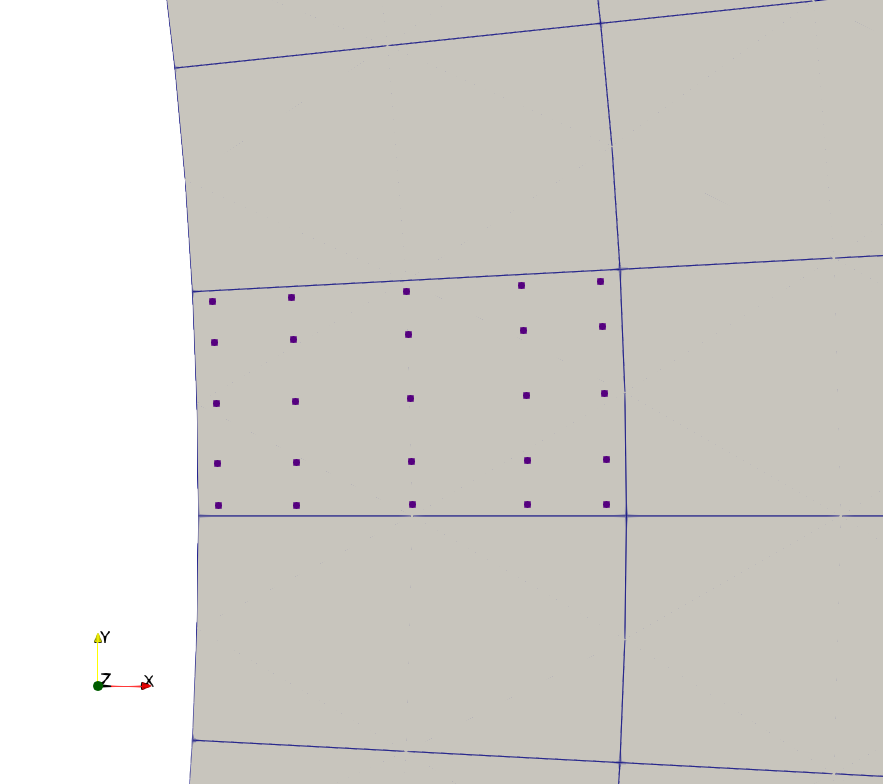
\includegraphics[width=4.2cm]{images/nq25}\\
{\captionfont Layout of the quadrature points in element \#0 of the mesh. 
From left to right: {\python nqperdim=2,3,4,5}.} 
\end{center}

Note that the {\python axisymmetric} flag controls whether the Stokes equations 
are solved in plane strain or under the assumption that there is axisymmetry. 
In the latter case the mesh is a demi-annulus in the $x>0$ half plane.

